\chapter{實驗結果} \label{se_6}
本章節對我們實作的TwoStepBFT共識版本的geth 進行測試。測試的節點皆是在Amazon EC2 t2.small上運行。t2.small 的硬體規格為1個虛擬CPU 與2GB 的記憶體。交易型態則是基本的以太坊轉帳交易。我們以交易的吞吐量Throughput(每秒共識多少筆交易量)與區塊的延遲性latency(完成一個區塊共識平均需要多少時間)與來衡量共識的效率。我們也測試共識演算法的延展性(Scalability),以瞭解當參與共識的節點數量變多時,共識效能會受到怎樣的影響。最後,我們將節點分散部屬在世界各地,讓該系統較貼近真實的應用場景。並且與同區域實驗比較。
\section{環境建設}\label{se_6}
在實驗裡所有的節點是互相連通的,即每個節點都會互相知道彼此的位置,因此我們的節點是呈現網狀連線
在佈署所有節點之後,我們先讓節點互相交易約15分鐘,讓交易存入交易池內,這讓共識時產生的區塊能夠塞滿足夠的交易。接下來將運行共識約一小時,並將結果紀錄下來。
\section{同資料中心吞吐量與延遲性測試}\label{se_6}
6.2我們將探討我們的演算法在同資料中心的實驗環境下,觀察吐量與延遲性的變化。我們將機器都運行於美國-奧勒岡資料中心。
對於測試基本的交易吞吐量與延遲性測試,我們透過控制創世區塊裡的GasLimit來控制單個區塊能包含的最大交易數量,區塊大小分別為每個區塊包含500、1000、4000、8000筆交易。實驗總共進行了五種節點數分別是16、30、60、80、100 個節點。
\begin{figure}[htp]
\centering
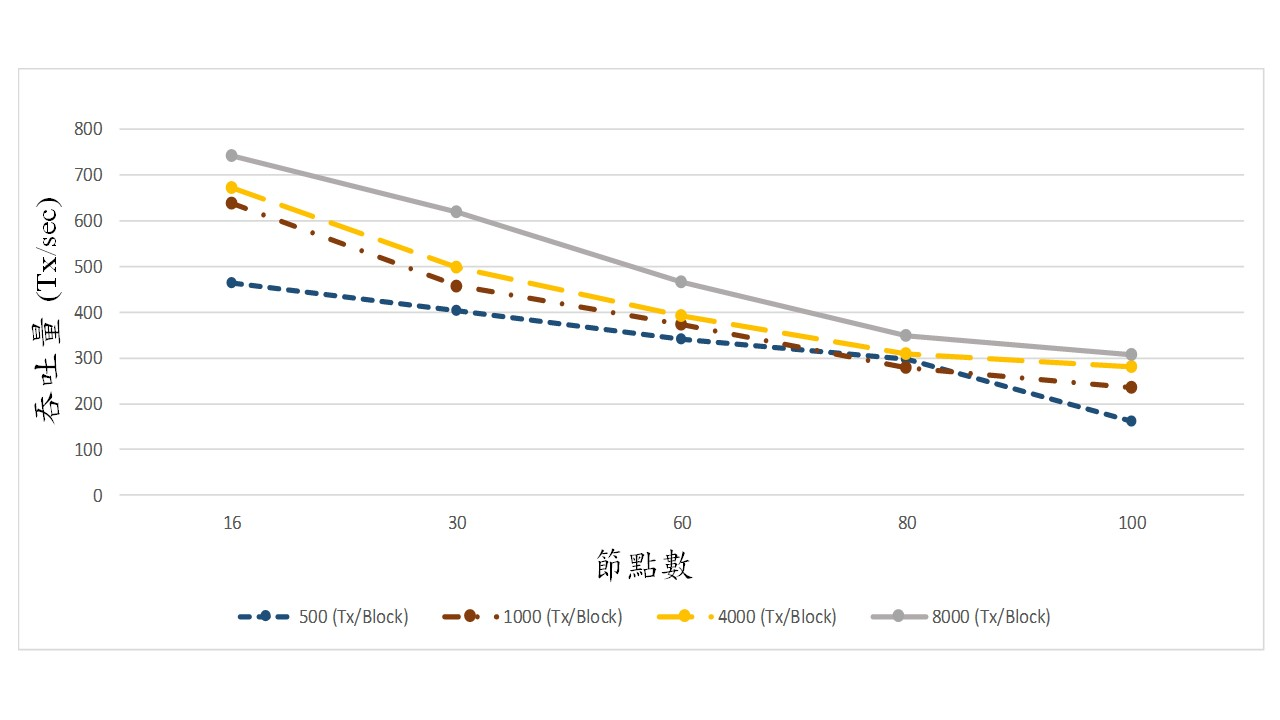
\includegraphics[scale=0.55]{images/61.png}
\caption{吞吐量 V.S 節點數}
\label{i:byz-latency}
\end{figure}
 
\newpage
\begin{figure}[h]
\centering
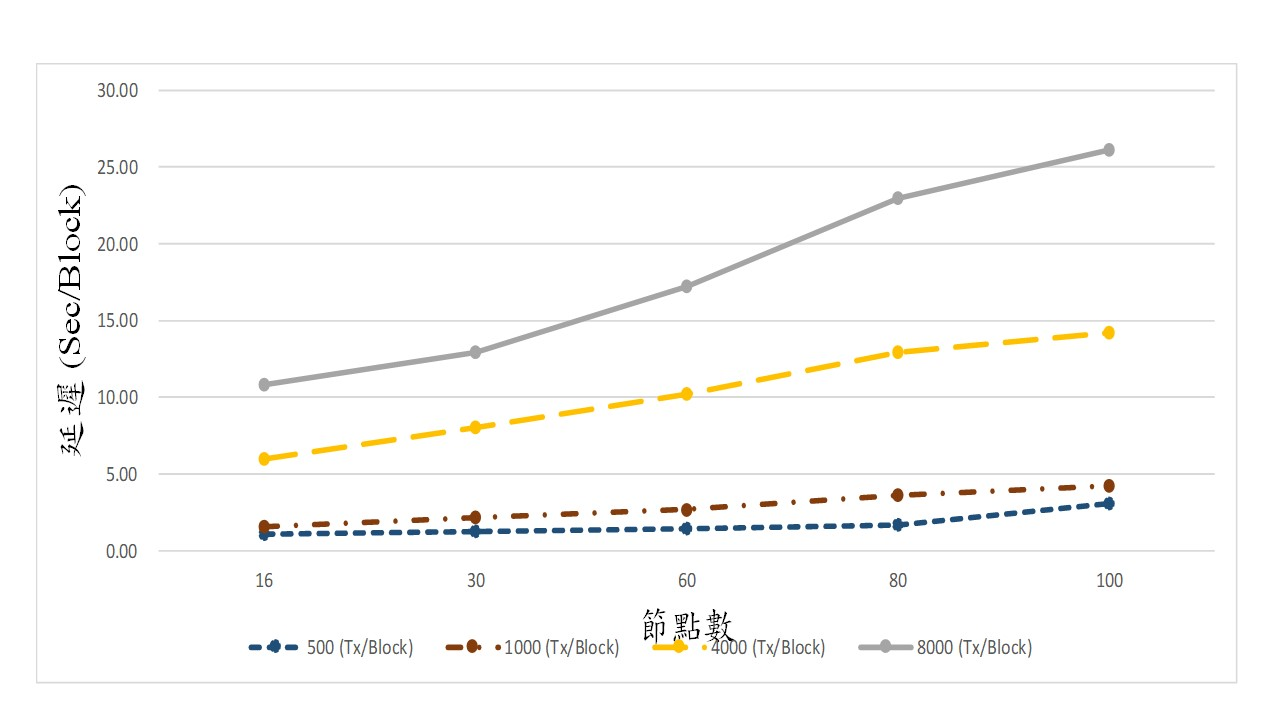
\includegraphics[scale=0.50]{images/62.jpg}
\caption{同資料中心的延遲性表現。}
\label{i:byz-latency}
\end{figure}


從圖6.1中可以看出在我們的共識演算法在節點數增加時,吞吐量隨之降低;而圖6.2則可以看出在我們的共識演算法在節點數增加時延遲也會隨之增加。當區塊大小增加時共識效率也會增加。且在100個節點吞吐量還能達到每秒300筆交易左右的共識速度,對於節點數的容忍能有良好的延展性。



\section{誇資料中心吞吐量與延遲性測試}\label{se_6}
6.3我們將探討我們的演算法在跨資料中心的實驗環境下,觀察吐量與延遲性的變化,並與同資料中心實驗進行比較。
與同區域的吞吐量與延遲性測試實驗一樣,我們先讓節點互相交易約15分鐘,讓交易存入交易池內,這讓共識時產生的區塊能夠塞滿足夠的交易。接下來將運行共識約一小時,並將結果紀錄下來。區塊大小分別為每個區塊包含500、1000、4000、8000筆交易。實驗總共進行了五種節點數分別是16、30、60、80、100 個節點。不同的是我們將節點分散的部屬在世界各地。這讓實驗更加貼近真實應用。在實驗裡我們將節點平均分散在(美國-奧勒岡、美國-維吉尼亞北部、日本-東京、新加玻、倫敦)
\begin{figure}[htp]
\centering
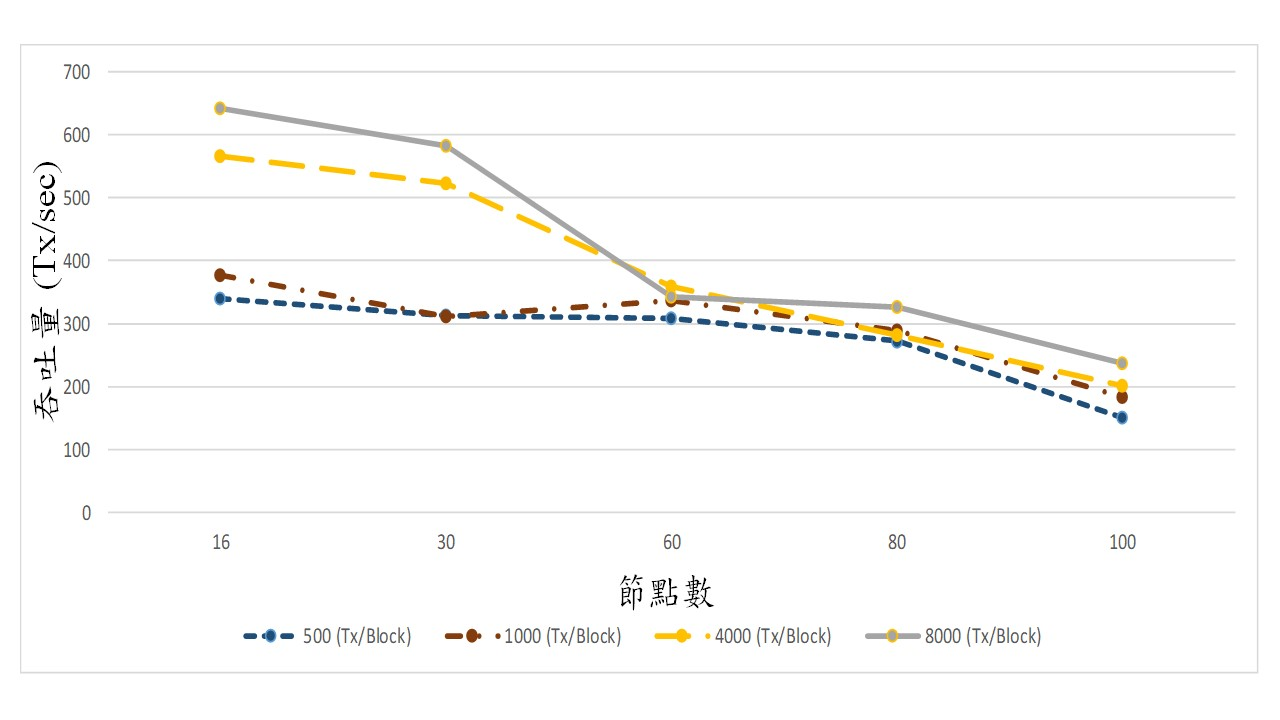
\includegraphics[scale=0.5]{images/63.jpg}
\caption{跨資料中心的交易吞吐量表現。}
\label{i:byz-latency}
\end{figure}

\begin{figure}[htp]
\centering
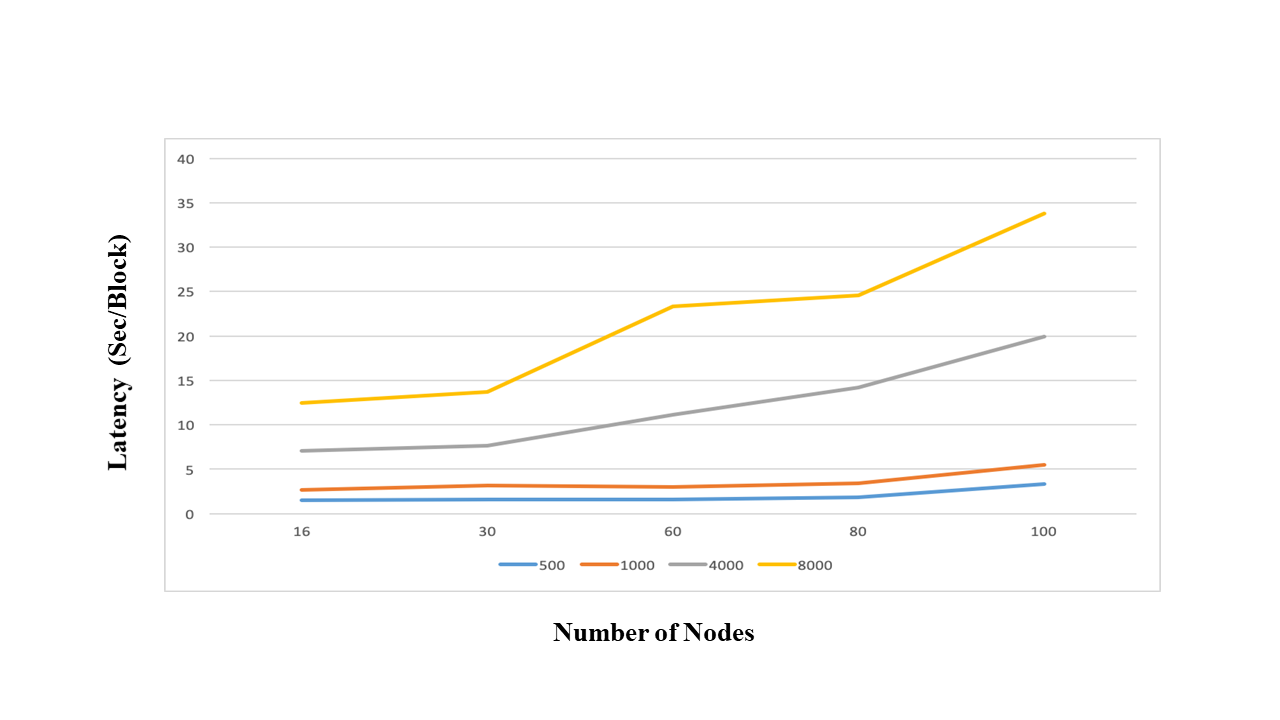
\includegraphics[scale=0.5]{images/64.jpg}
\caption{跨資料中心的延遲性表現。}
\label{i:byz-latency}
\end{figure}


在同區域的實驗裡,結果顯示在區塊大小為1000以上(Tx/Block)時,實驗結果穩定;但在區塊大小翻倍情況下,吞吐量並無大幅上升,但4000與8000的延遲卻大幅上升。也就是說在不同區域驗裡1000(Tx/Block)是一個較穩定的結果。從圖中也能觀察到在不同區域的實驗裡,吞吐量幾乎皆小於同區域的實驗,延遲也較同區域的實驗高。但即使在不同區域裡,100個節點的共識吞吐量也維持約有300TPS左右。

\begin{figure}[htp]
\centering
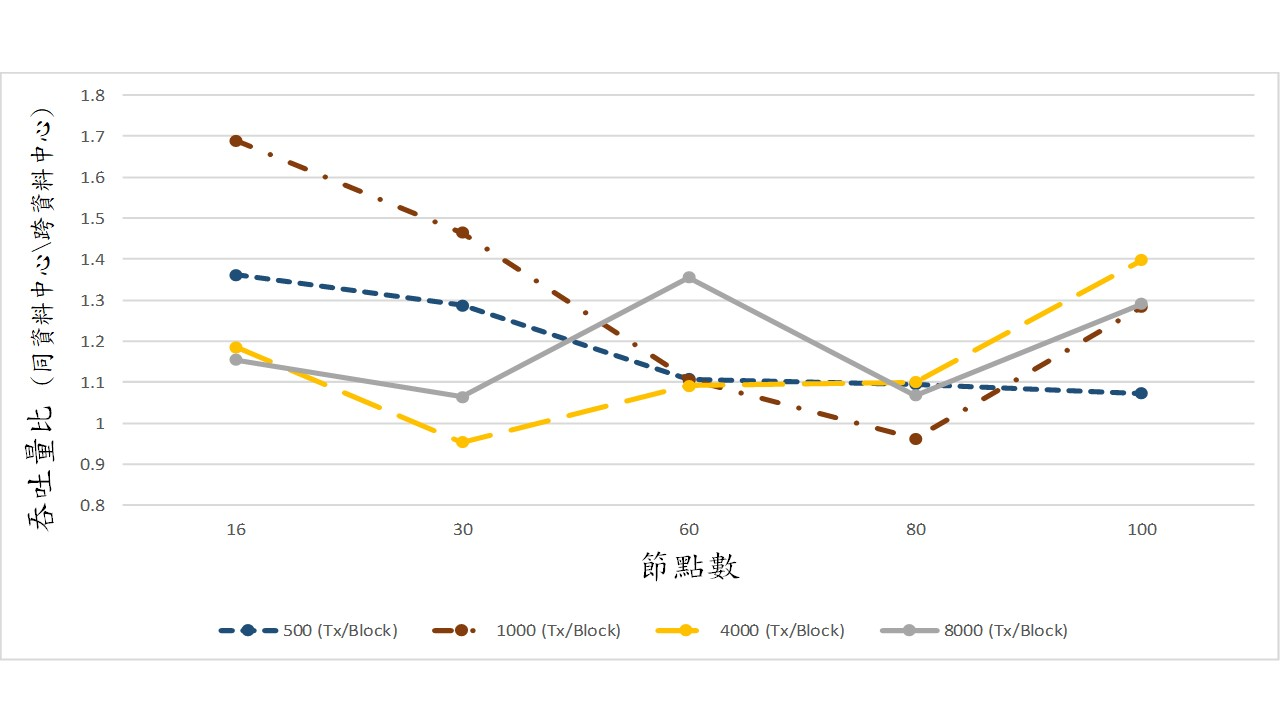
\includegraphics[scale=0.5]{images/65.jpg}
\caption{同資料中心與跨資料中心吞吐量比。}
\label{i:byz-latency}
\end{figure}

\begin{figure}[h]
\centering
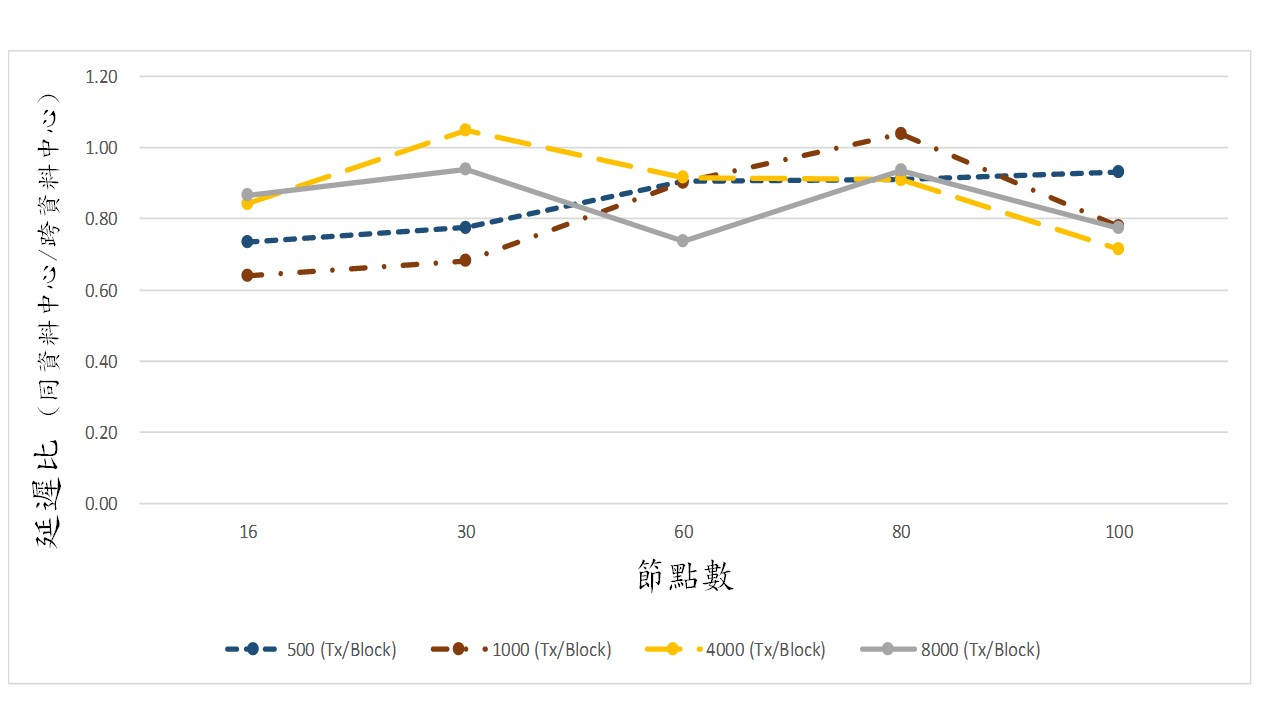
\includegraphics[scale=0.8]{images/66.jpg}
\caption{同資料中心與跨資料中心延遲比。}
\label{i:byz-latency}
\end{figure}


